% Copyright 2004 by Till Tantau <tantau@users.sourceforge.net>.
%
% In principle, this file can be redistributed and/or modified under
% the terms of the GNU Public License, version 2.
%
% However, this file is supposed to be a template to be modified
% for your own needs. For this reason, if you use this file as a
% template and not specifically distribute it as part of a another
% package/program, I grant the extra permission to freely copy and
% modify this file as you see fit and even to delete this copyright
% notice. 

\documentclass{beamer}


% There are many different themes available for Beamer. A comprehensive
% list with examples is given here:
% http://deic.uab.es/~iblanes/beamer_gallery/index_by_theme.html
% You can uncomment the themes below if you would like to use a different
% one:
%\usetheme{AnnArbor}
%\usetheme{Antibes}
%\usetheme{Bergen}
%\usetheme{Berkeley}
%\usetheme{Berlin}
%\usetheme{Boadilla}
%\usetheme{boxes}
%\usetheme{CambridgeUS}
%\usetheme{Copenhagen}
%\usetheme{Darmstadt}
\usetheme{default}
%\usetheme{Frankfurt}
%\usetheme{Goettingen}
%\usetheme{Hannover}
%\usetheme{Ilmenau}
%\usetheme{JuanLesPins}
%\usetheme{Luebeck}
%\usetheme{Madrid}
%\usetheme{Malmoe}
%\usetheme{Marburg}
%\usetheme{Montpellier}
%\usetheme{PaloAlto}
%\usetheme{Pittsburgh}
%\usetheme{Rochester}
%\usetheme{Singapore}
%\usetheme{Szeged}
%\usetheme{Warsaw}

\newcommand{\backupbegin}{
   \newcounter{framenumberappendix}
   \setcounter{framenumberappendix}{\value{framenumber}}
}
\newcommand{\backupend}{
   \addtocounter{framenumberappendix}{-\value{framenumber}}
   \addtocounter{framenumber}{\value{framenumberappendix}} 
}

\usepackage{hyperref}
\usepackage[utf8]{inputenc}
\usepackage[T1]{fontenc}
\usepackage[frenchb]{babel}
\usepackage{graphicx}
\usepackage{wrapfig}
\usepackage{caption}
\usepackage{subcaption}
\usepackage{natbib}
% Permet d'enlever les extensions
\DeclareGraphicsExtensions{.pdf,.png,.jpg}
% Dossier des images
\graphicspath{ {img/} }
% Taille des captions (texte sous images)
\usepackage[font={small,it}]{caption}
%\usepackage[linesnumbered]{algorithm2e}
\usepackage{float}

\newcommand{\whiteCircle}{\protect
\includegraphics[width=0.1\textwidth]{rond_blanc}}
\newcommand{\nun}{\protect\includegraphics[width=0.06\textwidth]{n1}}
\newcommand{\nd}{\protect\includegraphics[width=0.06\textwidth]{n2.pdf}}
\newcommand{\nq}{\protect\includegraphics[width=0.06\textwidth]{n4.pdf}}
\newcommand{\nc}{\protect\includegraphics[width=0.06\textwidth]{n5.pdf}}
\newcommand{\ns}{\protect\includegraphics[width=0.06\textwidth]{n6.pdf}}
\newcommand{\nse}{\protect\includegraphics[width=0.06\textwidth]{n7.pdf}}
\newcommand{\nh}{\protect\includegraphics[width=0.06\textwidth]{n8.pdf}}
\captionsetup[figure]{labelsep=period}
\title{
Construire et exploiter des croyances sur le monde à partir de régularités d'interactions expérimentées\\}
%Créer les mécanismes de représentation et d'utilisation d'objets du monde à partir de régularités d'interactions observées}

\author{Florian~Bernard}
% - Give the names in the same order as the appear in the paper.
% - Use the \inst{?} command only if the authors have different
%   affiliation.

\institute[Université Claude Bernard] % (optional, but mostly needed)
{
  
 Encadrant : Amélie Cordier \\
 Avec la participation d'Olivier Georgeon
}
% - Use the \inst command only if there are several affiliations.
% - Keep it simple, no one is interested in your street address.

\date{\today}
% - Either use conference name or its abbreviation.
% - Not really informative to the audience, more for people (including
%   yourself) who are reading the slides online

% This is only inserted into the PDF information catalog. Can be left
% out. 

% If you have a file called "university-logo-filename.xxx", where xxx
% is a graphic format that can be processed by latex or pdflatex,
% resp., then you can add a logo as follows:

% \pgfdeclareimage[height=0.5cm]{university-logo}{university-logo-filename}
% \logo{\pgfuseimage{university-logo}}

% Delete this, if you do not want the table of contents to pop up at
% the beginning of each subsection:
%\AtBeginSubsection[]
%{
%  \begin{frame}<beamer>{Outline}
%    \tableofcontents[currentsection,currentsubsection]
%  \end{frame}
%}

% Let's get started
\addtobeamertemplate{navigation symbols}{}{%
    \usebeamerfont{footline}%
    \usebeamercolor[fg]{footline}%
    \hspace{1em}%
    \insertframenumber/\inserttotalframenumber
}
\begin{document}

\begin{frame}
  \titlepage
\end{frame}

\begin{frame}{Sommaire}
  \tableofcontents
  % You might wish to add the option [pausesections]
\end{frame}

% Section and subsections will appear in the presentation overview
% and table of contents.
\section{Contexte}
\begin{frame}{Contexte}{Philosophique}
	E. Kant définit~:
	\begin{itemize}
		\item Monde nouménal~: le monde tel qu'il est
		\item Monde phénoménal~: le monde du point de vue de l'individu
	\end{itemize}
%		
%	E. Husserl introduit la phénoménologie en 1913~:
%	\begin{itemize}
%		\item Toute conscience doit être conçue comme conscience de quelque chose~\citep{phenomenologie-husserl}
%	\end{itemize} 
\end{frame}

\begin{frame}{Contexte}{Théorie de la cognition incarnée}
	\begin{figure}
		\includegraphics[width=\textwidth]{inverted_vs_traditionnal_model}
		\caption{Modèle du cycle Expérience/Résultat à gauche et classique à droite~\citep{georgeon2014inverting}}
%	\begin{subfigure}[b]{0.4\textwidth}
%		\includegraphics[width=\textwidth]{traditionnal_model}
%		\caption{Cycle observation/action traditionnel}
%	\end{subfigure}
%	\begin{subfigure}[b]{0.5\textwidth}
%		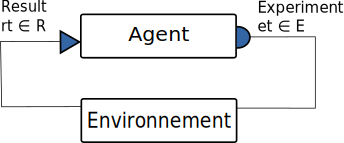
\includegraphics[width=\textwidth]{inverted_model}
%		\caption{Cycle expérience/résultat}
%	\end{subfigure}
	\end{figure}
	
	%TODO graphique pour apprentissage développemental. 
	L'agent est~:
	\begin{itemize}
		\item incarné~: il agit pour connaître son environnement~\citep{embodied-anderson2003embodied}
		\item agnostique~: les données d'entrée ne sont pas fonction de l'état du monde~\citep{Liris-5510-environment-agnostic}
	\end{itemize}
	Il utilise~:
	\begin{itemize}
		\item l'apprentissage développemental (schème sensorimoteur~\citep{cognitiviste-piaget1959construction})
		\item les interactions
	\end{itemize}
\end{frame}
\begin{frame}{Contexte}{Définition des interactions}
	\begin{itemize}
		\item Couple action/résultat
		\item Valence
	\end{itemize}
	\begin{figure}
		\centering
		\includegraphics[width=0.7\textwidth]{model_radical_interactionnism}
		\caption{Modèle basé sur les interactions}
	\end{figure}
\end{frame}

\section{Définition du problème}
\begin{frame}{Définition du problème}
\framesubtitle{Du point de vue de l'agent}
\begin{itemize}
\item Couplage entre l'agent et l'environnement à travers les interactions~:
\end{itemize}
\begin{figure}
\centering
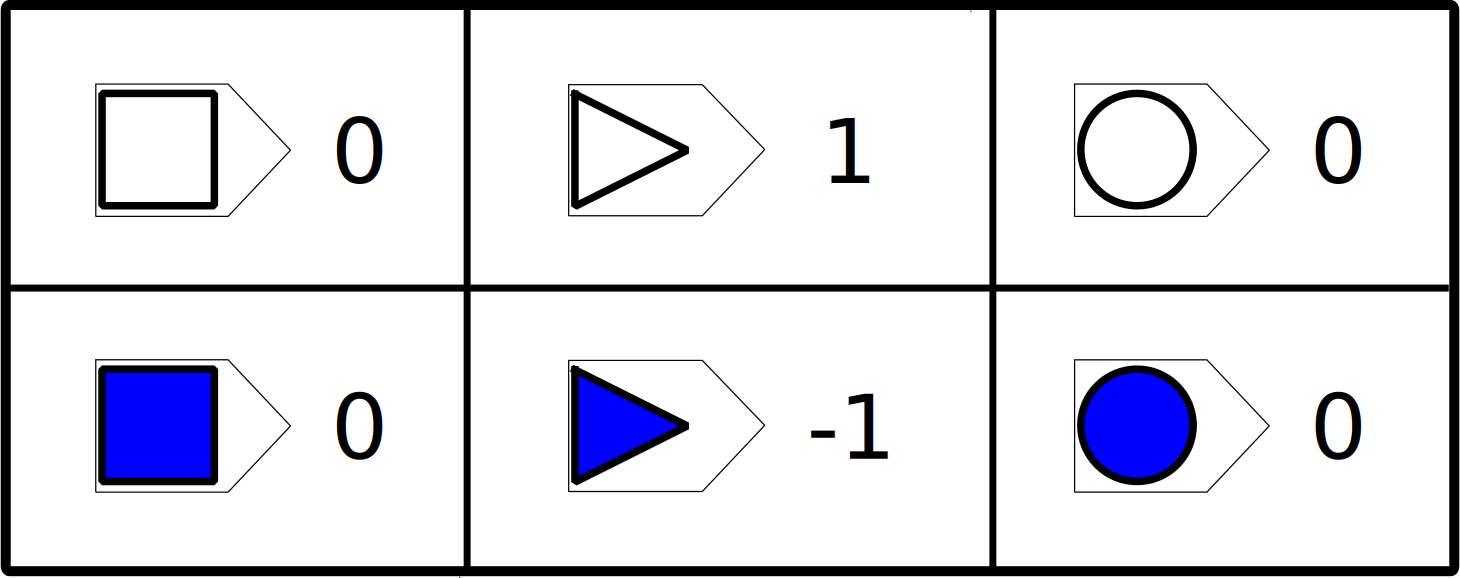
\includegraphics[width=0.15\textwidth]{interactions_string_problem}
\caption{L'agent est initialisé avec ces interactions}
\label{fig:listInteraction}
\end{figure}

%TODO changer le graph pour en avoir deux, le premier pour le flux d'interaction et le second pour les régularités imédiates dans le flux d'interaction (cadre autour des interaction)
\begin{figure}
\centering
\includegraphics[width=0.7\textwidth]{flux_interactions_hedonism_string_problem}
\caption{Flux d'interactions intended et enacted}
\label{fig:interactions_flux}
\end{figure}
\end{frame}


\begin{frame}{Définition du problème}{Régularités}
	%TODO Changer le graphe. À voir si je ne met pas le flux avec les régularités puis les régularités interassantes.
\begin{figure}
	\centering
	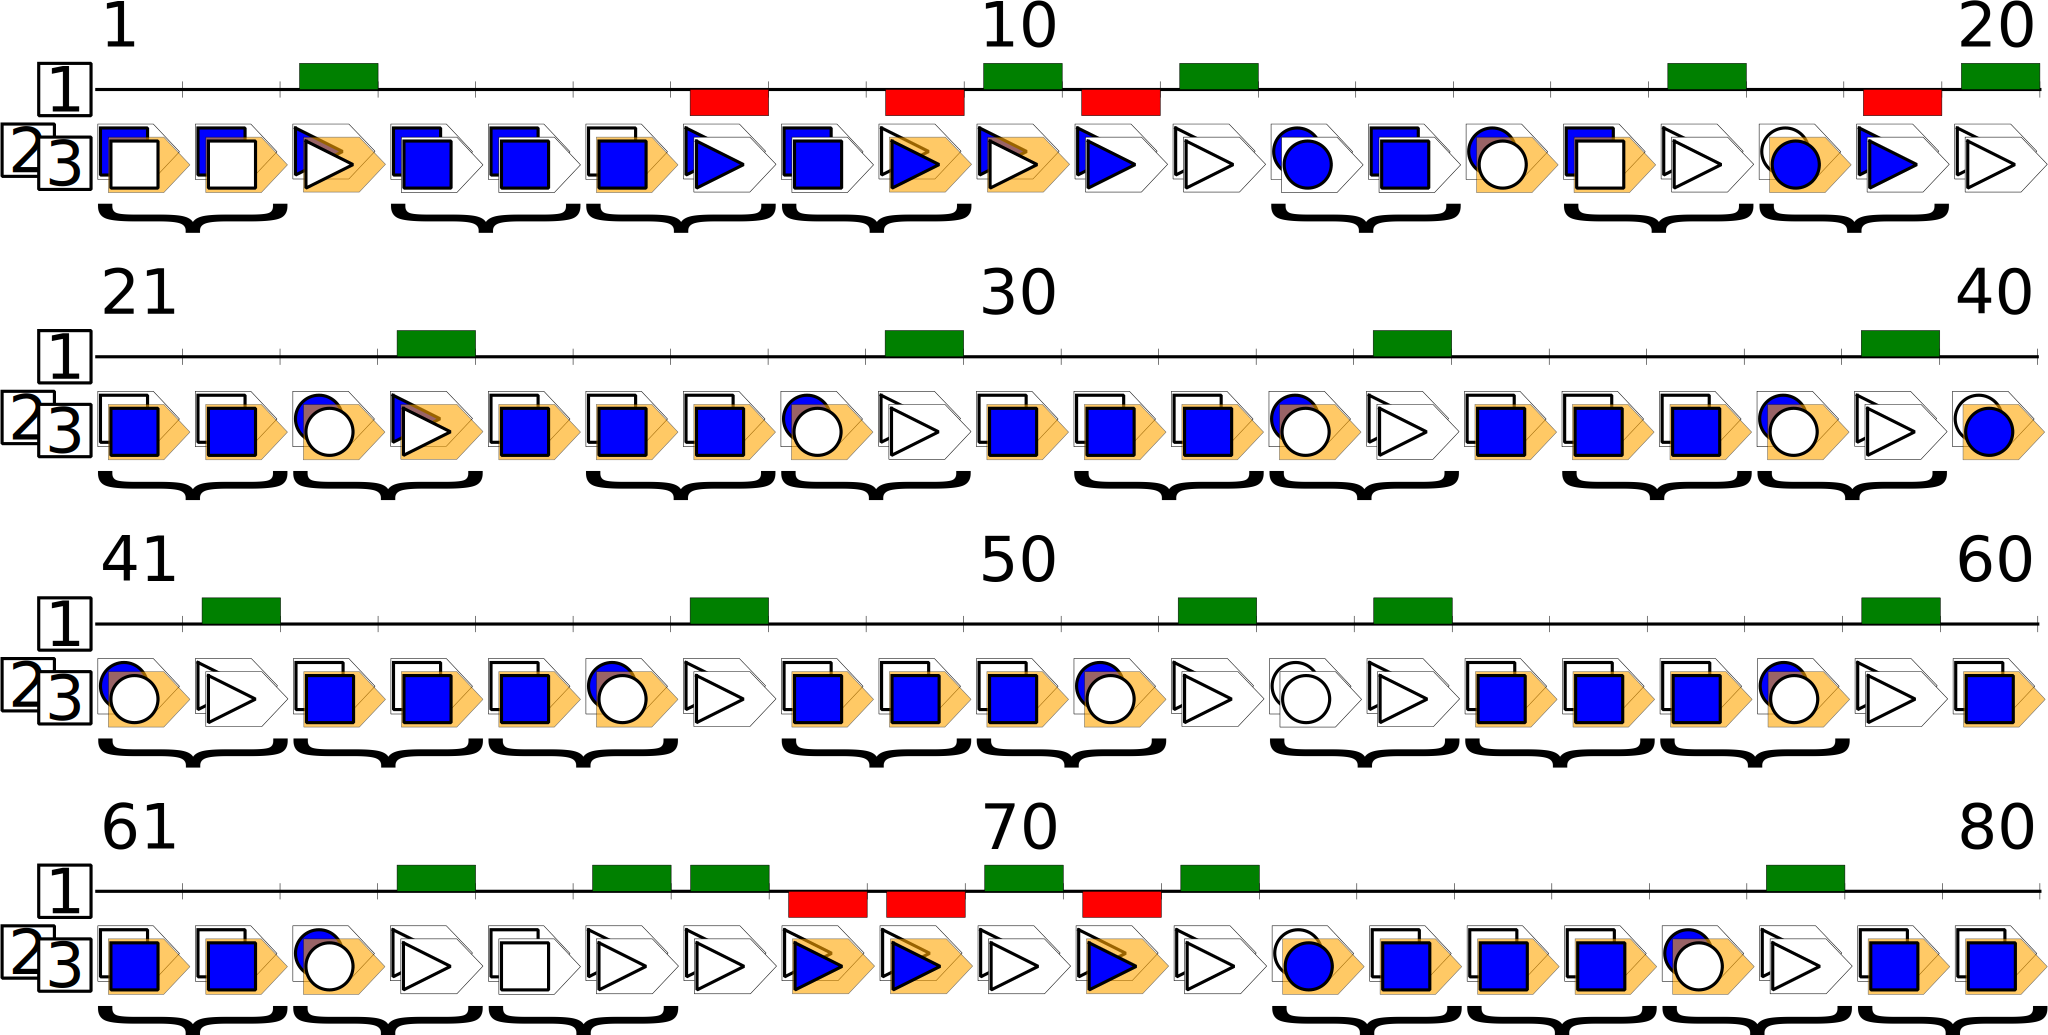
\includegraphics[width=0.9\textwidth]{flux_interactions_with_regularities_hedonism_string}
\end{figure}
\begin{figure}
	\centering
	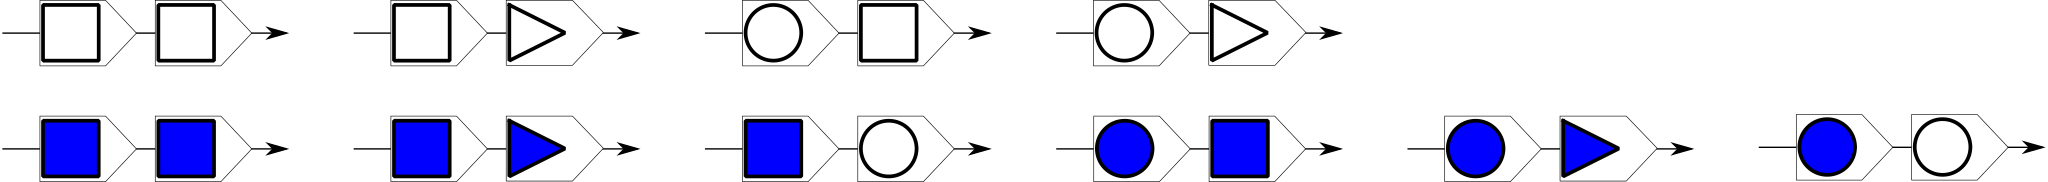
\includegraphics[width=0.9\textwidth]{regularities_string_problem}
	\caption{Régularités disponibles dans l'environnement}
\end{figure}
\end{frame}
\begin{frame}{Définition du problème}{Régularités}
	\begin{figure}
		\centering
		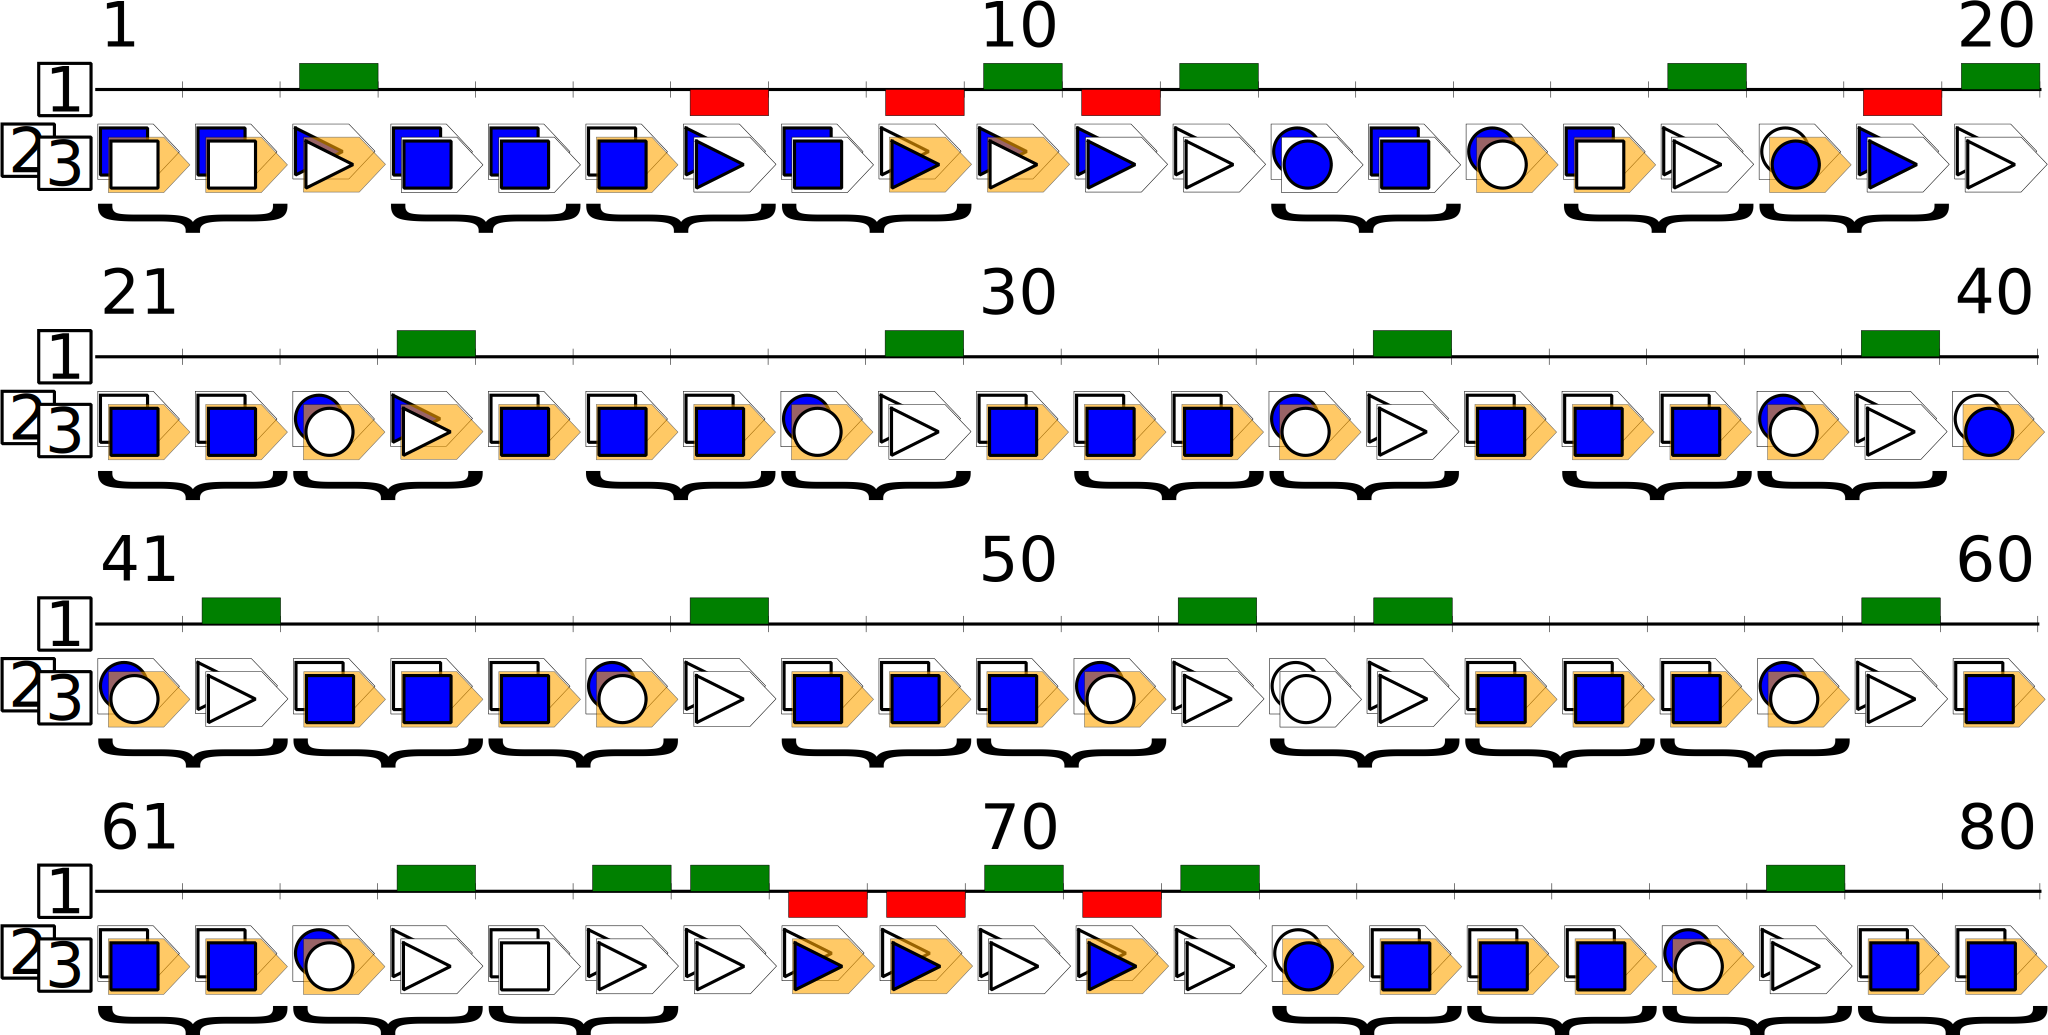
\includegraphics[width=0.9\textwidth]{flux_interactions_with_regularities_hedonism_string}
	\end{figure}
\begin{figure}
	\centering
	\includegraphics[scale=0.06]{well_regularities_string_problem}
	\caption{Régularités séquentielles que l'on souhaiterait que l'agent trouve et utilise pour satisfaire sa motivation}
\end{figure}
\end{frame}

\begin{frame}{Définition du problème}{Environnement \emph{String problem}}
%	\begin{figure}
%		 \includegraphics[width=0.8\textwidth]{string_problem_1}
%	\end{figure}
	\begin{figure}
		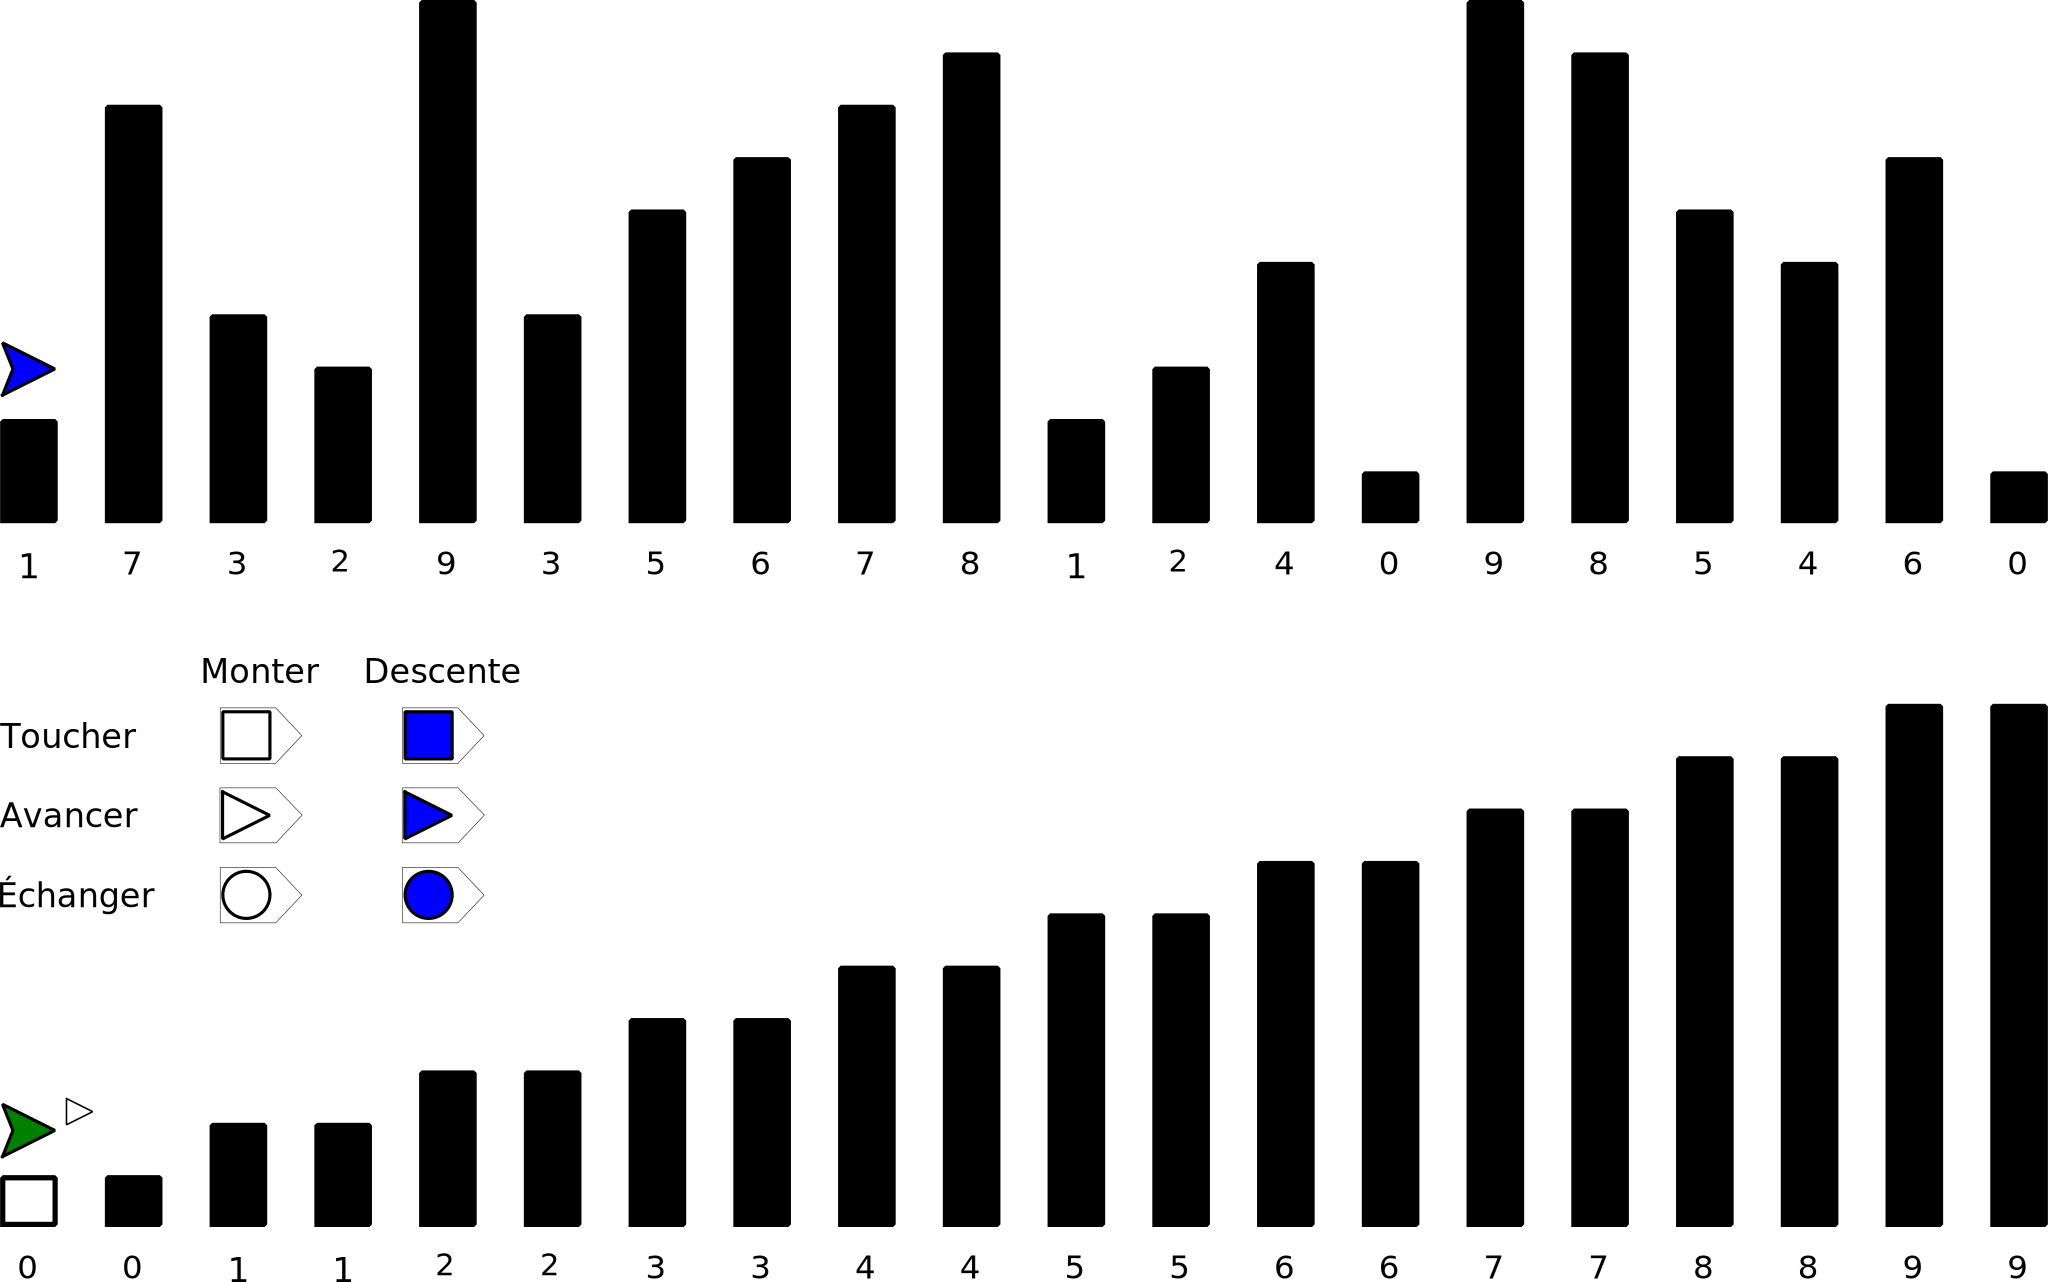
\includegraphics[width=0.8\textwidth]{string_human}
		\caption{Représentation graphique du monde nouménal~\citep{Liris-6368-string-problem}}
	\end{figure}
	%TODO graphic, chaine de digit + interaction pour qu'ils comprennent les liens entre interactions et les actions.
\end{frame}
\section{Contributions}

%\begin{frame}{Modèle et structures utilisées}{Radical Interactionism}
%% Graphics d'interaction composite
%\begin{figure}
%\centering
%\includegraphics[width=0.6\textwidth]{radicalInteractionnism}
%\caption{Diagramme d'implémentation}
%\label{fig:radicalInteractionnism}
%\end{figure}
%\end{frame}

\begin{frame}{Contributions}{Table d'usage d'interaction}
%TODO voir pour incorporé le graph des tables d'usage ici.

%\begin{itemize}
%	\item Concept des signatures
%	\item Maintenir à jour le nombre d'intended et d'enacted pour chaque:
%	\begin{itemize}
%		\item Pré-interaction
%		\item Post-interaction
%		\item Alternative
%		\item Opposée
%	\end{itemize}
%	\item Persistante
%	\item Sporadique
%	\item Sporadique avec croyance
%\end{itemize}
\begin{minipage}[0.4]{\textwidth}
	\begin{columns}[T]
		\begin{column}{0.5\textwidth}
			\begin{itemize}
				\item Concept des signatures~\citep{simon}
				\item Maintenir à jour le nombre d'intended et d'enacted pour chaque:
				\begin{itemize}
					\item \ns Pré-interactions
					\item \nh Post-interactions
					\item \nse Alternatives
					\item \nse Opposées
				\end{itemize}
				\item \nd Types~:
				\begin{itemize}
					\item Persistante
					\item Sporadique
					\item Sporadique avec croyance
				\end{itemize}
			\end{itemize}
		\end{column}
		\begin{column}{0.4\textwidth}
			\begin{figure}
			\includegraphics[width=\textwidth]{usage_table_white_circle_string_problem}
			\caption{Table d'usage de l'interaction \whiteCircle~: \og~\emph{swap up}~\fg}
			\end{figure}
		\end{column}
	\end{columns}
\end{minipage}
\end{frame}

%\begin{frame}{Modèle et structures utilisées}{Table d'usage d'interaction}
%\begin{figure}
%\centering
%\includegraphics[height=0.7\textheight]{usageTable}
%\caption{Table d'usage de l'interaction feelDown}
%\label{fig:usageTable}
%\end{figure}
%\end{frame}

\begin{frame}{Contributions}{État de croyance interne}
\begin{itemize}
\item Inconnu~: interaction sporadique avec ou sans croyance
\item Phénomène~: interaction persistante
\end{itemize}
\begin{figure}
\centering
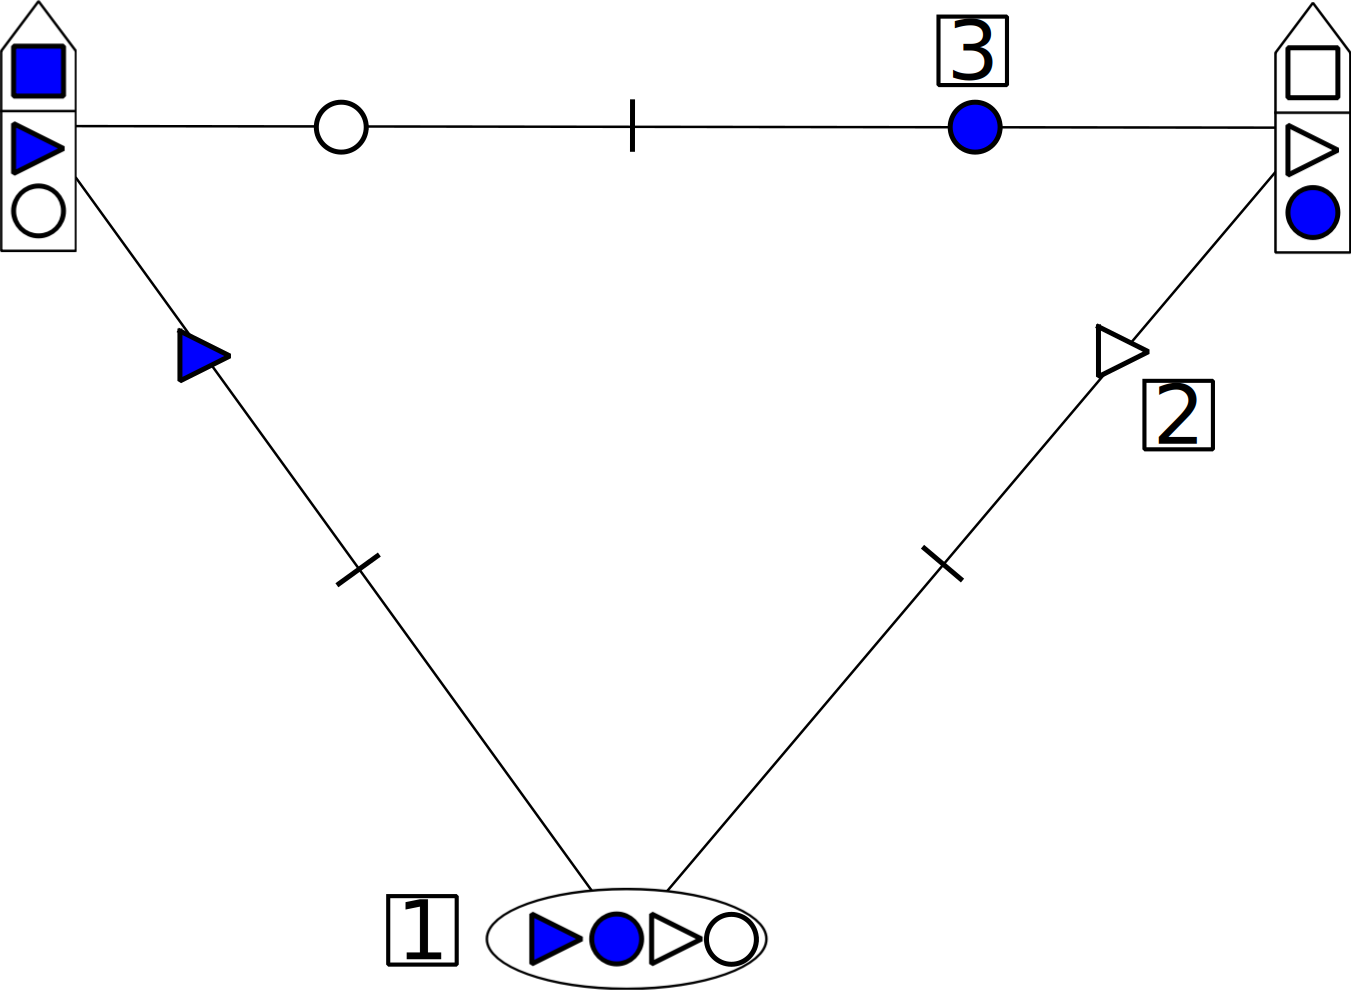
\includegraphics[width=0.5\textwidth]{petri_hedonism_string_problem}
\caption{Représentation des convictions de l'agent}
\label{fig:internalObjects}
\end{figure}
\end{frame}
\section{Démonstration}
\begin{frame}{Démonstration}

\end{frame}

\begin{frame}{Interactionnisme radical}
\begin{figure}
	\centering
	\includegraphics[scale=0.5]{radical_interactionnism}
	\caption{Modèle de l'interactionnisme radical}
\end{figure}
%\begin{itemize}
%	\item Interaction primitive
%	\item Interaction composite
%	\begin{itemize}
%		\item Pré-interaction
%		\item Post-interaction
%	\end{itemize}
%\end{itemize}
\end{frame}

\begin{frame}{Démonstration}
\end{frame}
%\begin{frame}{Phénomènes persistants appris par l'agent}
%	\begin{figure}
%		\centering
%		\includegraphics[height=0.4\textheight]{internalBelieve}
%		%\caption{Structure d'un phénomène appris}
%		\label{fig:phenomene}
%	\end{figure}
%	
%	\begin{figure}
%		\centering
%		\includegraphics[height=0.4\textheight, width=\textwidth]{interactions_with_believe}
%		%\caption{Flux d'interaction}
%		\label{fig:flux_interaction}
%	\end{figure}
%\end{frame}

%TODO faire les algo en français sous forme de diagramme.
%\section{Algorithmes}

%\begin{frame}{Apprentissage et exploitation}
%\begin{algorithm}[H]
%\SetAlgoLined
%\DontPrintSemicolon
%\While{Existence}{
%    intended $\leftarrow$ decision.getIntend()\;
%    enacted $\leftarrow$ action.tryToExecute(intended)\;
%    updateUsageTable(intended, enacted)\;
%    decision.hasEnacted(enacted)\;
%}
%\end{algorithm}
%\end{algorithm}
%\end{frame}
%\begin{frame}{Algorithmes}
%	\begin{figure}
%		\centering
%		\includegraphics[scale=0.35]{intended_enacted_1}
%	\end{figure}
%\end{frame}
%\begin{frame}{Algorithmes}
%	\begin{figure}
%		\centering
%		\includegraphics[scale=0.34]{intended_enacted_2}
%	\end{figure}
%\end{frame}
%\begin{frame}{Algorithmes}
%
%\begin{figure}
%	\centering
%	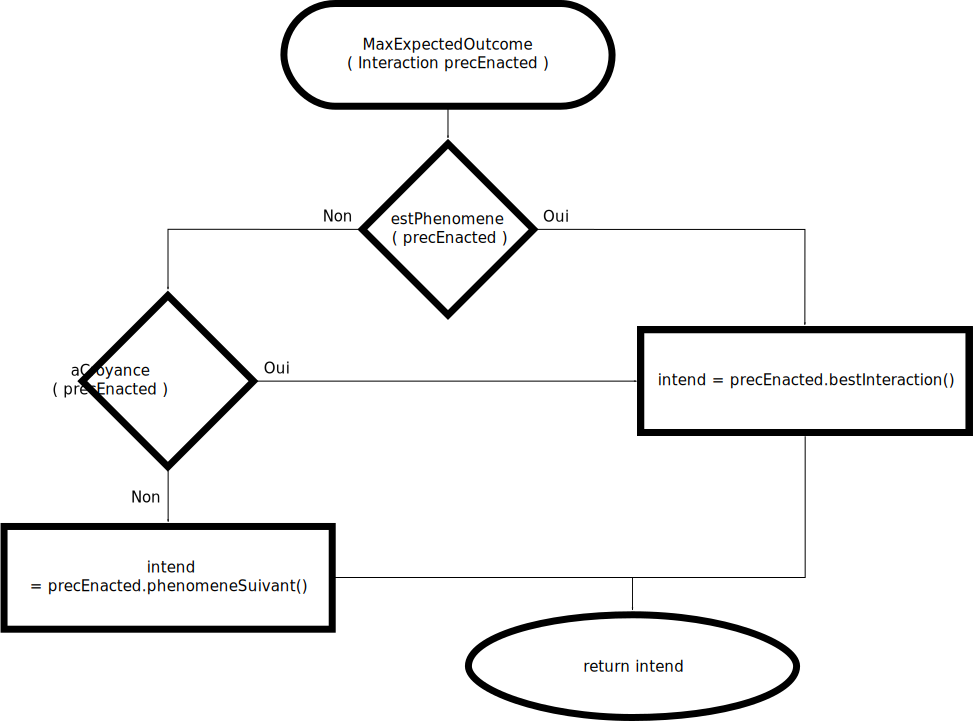
\includegraphics[width=\textwidth]{max_outcome}
%\end{figure}
%\begin{algorithm}[H]
%\SetAlgoLined
%\DontPrintSemicolon
%\SetKwFunction{FGetIntend}{getIntend}
%\SetKwProg{Func}{Function}{}{}
%Believe $\leftarrow$ "unknown"\;
%mood $\leftarrow$ "curious"\;
%\Func{\FGetIntend{}}
%{
%    \eIf {mood $=$ "curious"} {
%        intended $\leftarrow$ leastTriedExperiment(Believe) \;
%    }{
%        \eIf{mood $=$ "hedonist"} {
%            intended $\leftarrow$ intendedMaxExpectedOutcomeValence(Believe)\;
%        } {
%            \If{mood $=$ "excited"} {
%                intended $\leftarrow$ lastEnacted\;
%            }
%        }
%    }
%    \KwRet intended\;
%}
%\BlankLine
%\end{algorithm}
%\end{frame}

%\begin{frame}
%\begin{algorithm}[H]
%\scriptsize
%\SetAlgoLined
%\DontPrintSemicolon
%\SetKwFunction{FHasEnacted}{hasEnacted}
%\SetKwProg{Proc}{Procedure}{}{}
%\Proc{\FHasEnacted{Interaction enacted}}
%{
%    \If {mood $=$ "excited"} {
%        \eIf{enacted $\ne$ lastEnacted} {
%            enacted.setUnpersistent()\;
%        } {
%            \eIf{excitement $>$ excitementThreshold} {
%                enacted.setPersistent()\;
%            } {
%                excitement ++\;
%            }
%        }
%    }
%    Believe $\leftarrow$ updateAndGetBelieve(intended, enacted)\;
%    \If {mood $\ne$ excited} {
%        mood $\leftarrow$ "hedonist"\;
%    } 
%    \eIf {enacted.isUnknown()} {
%        mood $\leftarrow$ "excited"\;
%        lastEnacted $\leftarrow$ enacted\;
%    } {
%        \If {all the experiments have not been tried yet in the context of believe} {
%            mood $\leftarrow$ "curious"\;
%        }
%    }
%    \KwRet\;
%}
%\end{algorithm}
%\end{frame}
%
%\begin{frame}{}
%\begin{algorithm}[H]
%\scriptsize
%\SetAlgoLined
%\DontPrintSemicolon
%\SetKwFunction{FIntendedMaxExpectedOutcomeValence}{intendedMaxExpectedOutcomeValence}
%\SetKwProg{Func}{Function}{}{}
%\Func{intendedMaxExpectedOutcomeValence{TableInteractions believe}} {
%    \eIf{isPhenomena(believe)} {
%        \ForEach{interactionLine $e$ of believe.getPostInteraction()}{
%            \If{$e$.isConfirm()} {
%                addAnticipation($e$.getInteraction()\;
%                    \Indp , $e$.getReward()\;
%                    , $e$.getFactor()\;
%                    )\;
%            }
%        }
%    } {
%        \eIf{believe.hasBelieve()}{
%            intendedMaxExpectedOutcomeValence(believe.getBelieve())\;
%        } {
%            \ForEach{interactionLine $e$ of believe.getPostInteraction()}{
%                \If{$e$.isPhenomena()}{
%                    addAnticipation($e$.getInteraction()\;
%                       \Indp , $e$.getReward()\;
%                        , $e$.getFactor()\;
%                }
%            }
%        }
%        
%    }
%    \KwRet bestInteractionInAnticipation()\;
%}
%\end{algorithm}
%\end{frame}

\section{Synthèse du point de vue de l'agent}
\begin{frame}{Synthèse du point de vue de l'agent}{Ce que l'agent sait faire}
\begin{itemize}
\item Trouver les régularités directes et indirectes des interactions
\item Construire et maintenir des phénomènes
\item Naviguer dans des environnements simples 
\end{itemize}
\end{frame}

\begin{frame}{Synthèse du point de vue de l'agent}{Perspectives}
\begin{itemize}
\item Apprendre des régularités séquentielles hiérarchiques (séquences et sous-séquences)
\item Apprendre des interactions composites pour atteindre le modèle de l'interactionnisme radical~\citep{Liris-6480-radical-interactionism}
\item Créer des phénomènes à partir d'interactions composites
\item Est-ce que l'agent pourra appréhender des environnements spatiaux avec uniquement des phénomènes et des interactions composites ?
\end{itemize}
\end{frame}

%\section{Références}
%\begin{frame}[plain, allowframebreaks]{Références}
%	\pagenumbering{gobble}
%	
%\end{frame}
\section{Questions}
\begin{frame}[plain]{Des questions ?}

\end{frame}

\backupbegin
\begin{frame}[plain, allowframebreaks]{Références}
\bibliographystyle{authordate1}
\bibliography{bibliographie}
\end{frame}
\backupend
\end{document}


